\documentclass[11pt,a4paper,oneside,french,svgnames]{report}
\usepackage[utf8]{inputenc} % force the use of utf8
\usepackage[T1]{fontenc} % font encoding, allows accents
\usepackage[papersize={21cm,29.7cm},top= 2.5cm,bottom=2.5cm, inner=2.5cm, outer=2.5cm]{geometry} % page formatting
\usepackage[francais]{babel} % translate everything in the desired language: table of contents, etc. 'english' can be replaced with 'francais'
\usepackage{graphicx} % images management
\usepackage{wrapfig} % floating images
\usepackage{array} % allow arrays
\usepackage{fancyhdr} % headers/footers management (overrides empty, plain and headings)
\usepackage{listings} % code insertion (MUST BE WRITTEN AFTER BABEL)
\usepackage{algpseudocode}
%\usepackage[nottoc,numbib]{tocbibind} % bib in toc
%\usepackage{pdfpages} % include PDF documents
\usepackage{enumitem} % for /setlist
\usepackage{subscript} % for \textsubscript
\usepackage{color,soul} % add some colors and hightlight
\usepackage{xcolor} % more colors
\usepackage[hyphens]{url} % auto break lines in URL
\usepackage{amsmath}
\usepackage[hidelinks,  colorlinks  = true, % no borders, colors enabled
                        anchorcolor = blue,
                        linkcolor   = black, % links in table of contents
                        urlcolor    = blue,
                        citecolor   = blue]{hyperref}
%\usepackage[%nonumberlist,% no page number
%            toc,% displayed in toc
%            numberedsection,% displayed as a numbered section in toc
%            xindy]{glossaries} % glossary with xindy style. MUST BE WRITTEN AFTER HYPERREF
%\setglossarystyle{listgroup}

\sethlcolor{cyan} % package soul
\newcommand{\file}[1]{\hl{\emph{#1}}} % highlight a file URI
\newcommand{\deriv}{\mathrm{d}}
%\makeglossaries
%\loadglsentries{glossary.tex}

%%%%%%%%%%%%%%%%%%%%%%%%%%%%%%%%%%%%%%%%%%%%%%%%%%%%%%%% LISTINGS %%%%%%%%%%%%%%%%%%%%%%%%%%%%%%%%%%%%%%%%%%%%%%%%%%%%%%%%
\definecolor{comment}{rgb}{0.12, 0.38, 0.18 } % adjusted, in Eclipse: {0.25, 0.42, 0.30 } = #3F6A4D
\definecolor{keyword}{rgb}{0.37, 0.08, 0.25}  % #5F1441
\definecolor{string}{rgb}{0.06, 0.10, 0.98} % #101AF9

\lstset{
  columns=flexible, %prevent extra spaces
  rulecolor=\color{black!50},
  backgroundcolor = \color{blue!10},
  numbers=none, % line numbering
  showspaces=false,
  showtabs=false,
  tabsize=2,
  breaklines=true,
  showstringspaces=false,
  breakatwhitespace=false,
  commentstyle=\color{comment},
  keywordstyle=\color{keyword},
  stringstyle=\color{string},
  basicstyle=\ttfamily,
  extendedchars=true,
  emph=[2]{In},
  emphstyle=[2]\color{black!70},
  morecomment=[l][\color{blue}]{Out},
  frame=single,
  frameround=tttt,
  framerule=0.3pt,
  framesep=4pt,
  belowcaptionskip=2.1pt,
  literate={à}{{\`a}}1 {à }{{\`a} }1 {â}{{\^a}}1 %           letter a
           {À}{{\`A}}1 {Â}{{\^A}}1 %                         letter A
           {ç}{{\c{c}}}1 %                                   letter c
           {Ç}{{\c{C}}}1 %                                   letter C
           {é}{{\'e}}1 {è}{{\`e}}1 {ê}{{\^e}}1 {ë}{{\"e}}1 % letter e
           {É}{{\'E}}1 {È}{{\`E}}1 {Ê}{{\^E}}1 {Ë}{{\"E}}1 % letter E
           {î}{{\^i}}1 {ï}{{\"i}}1 %                         letter i
           {Î}{{\^I}}1 {Ï}{{\"I}}1 %                         letter I
           {ô}{{\^o}}1 %                                     letter o
           {Ô}{{\^O}}1 %                                     letter O
           {œ}{{\oe}}1 %                                     letter oe
           {Œ}{{\OE}}1 %                                     letter OE
           {ù}{{\`u}}1 {û}{{\^u}}1 {ü}{{\"u}}1 %             letter u
           {Ù}{{\`U}}1 {Û}{{\^U}}1 {Ü}{{\"U}}1 %             letter U
  % above is a hack to force UTF8 compatibility (only for french)
}

\newcommand{\textcode}[1]{\lstset{
  language=,
  title={{\setlength{\fboxsep}{1pt}\fcolorbox{orange}{yellow!20}{\sffamily\scriptsize
              \textcolor{gray!10}{\_}{#1}\textcolor{gray!10}{\_}}}}
  }
}

\newcommand{\cpp}{\lstset{
  language=C++,
  title={{\setlength{\fboxsep}{1pt}\fcolorbox{orange}{yellow!20}{\sffamily\scriptsize
              \textcolor{gray!10}{\_}C++\textcolor{gray!10}{\_}}}}
  }
}

%%%%%%%%%%%%%%%%%%%%%%%%%%%%%%%%%%%%%%%%%%%%%%%%%%%%%%%%%%%%%%%%%%%%%%%%%%%%%%%%%%%%%%%%%%%%%%%%%%%%%%%%%%%%%%%%%%%%%%%%%%%

%\parindent=20pt
\fancypagestyle{plain}{
    % Headers
    \fancyhead[R]{Rapport TP5 SY31}
    \fancyhead[L]{\textsc{PELLERIN} - \textsc{PICHOU} - \textsc{SHI} - \textsc{SOEROPAIMAN}}

    % Footers
    \renewcommand{\footrulewidth}{0.1pt}
    \fancyfoot[C]{Université de Technologie de Compiègne}
    \fancyfoot[LE]{\ifnum\thepage>0 \thepage \fi}
    \fancyfoot[RO]{\ifnum\thepage>0 \thepage \fi}
}

\fancypagestyle{empty}{%
    \renewcommand{\headrulewidth}{0pt} % No sub line
    \fancyhead{} % Empty the header

    \renewcommand{\footrulewidth}{0pt}
    \fancyfoot{}
} 

\setlist[itemize,2]{label={$\bullet$}} % use bullets for nested itemize

% First page
\newcommand{\presentation}[1]{\vspace{0.3cm}\large{\textbf{#1}}\vspace{0.3cm}\\}
\newcommand{\presentationLarge}[1]{\vspace{0.3cm}\LARGE{\textbf{#1}}\vspace{0.3cm}\\}

% Overrides chapter (numbered and no-numbered) headings: remove space, display only the title
\makeatletter
  \def\@makechapterhead#1{%
  \vspace*{0\p@}% avant 50
  {\parindent \z@ \raggedright \normalfont
    %\ifnum \c@secnumdepth >\m@ne
    %    \huge\bfseries \@chapapp\space \thechapter
    %    \par\nobreak
    %    \vskip 20\p@
    %\fi
    \interlinepenalty\@M
    \Huge \bfseries \thechapter\quad #1   
    \vskip 40\p@
  }}
  \def\@makeschapterhead#1{%
  \vspace*{0\p@}% before 50
  {\parindent \z@ \raggedright
    \normalfont
    \interlinepenalty\@M
    \Huge \bfseries  #1\par\nobreak
    \vskip 40\p@
  }}
\makeatother

\newcommand{\ignore}[1]{} % inline comments

\pagenumbering{arabic}
%\addtocounter{page}{-7} % page numbering starts at 1 + (-7)
\pagestyle{plain} % uses fancy

\title{Rapport SY31}
\author{Romain PELLERIN, Kyâne PICHOU, Nianfei SHI et Ibraim SOEROPAIMAN}
\date\today

%\setcounter{tocdepth}{4}

\begin{document}
\thispagestyle{empty} % only for the current page

\begin{center}

\includegraphics[height=3cm]{UTC_logo.png}\\
\vspace{2.5cm}
\presentation{Université de Technologie de Compiègne} 
\presentation{SY31}

\vspace{2cm}
\noindent\fbox{
\begin{minipage}{0.9\textwidth}
\begin{center}
    \presentationLarge{Rapport de TP}
    \presentationLarge{\Huge{5 - Traitements d'images}}
\end{center}
\end{minipage}}
\vspace{3cm}

\presentation{Automne 2014}
\vspace{1cm}

\def\arraystretch{1.5} % 1 is the default
\begin{tabular}{|>{\hfill\arraybackslash}p{5cm}|p{5cm}|}
\hline
    \multicolumn{2}{|c|}{Romain \textsc{PELLERIN} - Kyâne \textsc{PICHOU} - Nianfei \textsc{SHI} - Ibraim \textsc{SOEROPAIMAN}}\\
\hline
     \multicolumn{2}{|c|}{Groupe de TP 2}\\% dates
\hline
    \multicolumn{2}{|c|}{\textit{\today}}\\% dates
\hline
\end{tabular}
\end{center}

\tableofcontents

\chapter{Introduction}
\section{Résumé}
L'objectif de ce TP est d'écrire un programme permettant la gestion d'une ludothèque composée de jeux de société. Un jeu de société est décrit par une fiche contenant les informations suivantes :
\begin{itemize}
  \item Nom du jeu
  \item Genre du jeu : PLATEAU, RPG, COOPERATIF, AMBIANCE ou HASARD
  \item Le nombre de joueurs minimum
  \item Le nombre de joueurs maximum
  \item La durée moyenne d'une partie en minutes
\end{itemize}

\section{Structuration du projet}
Nous avons choisi de structuer notre projet en 5 fichiers pour une meilleure clarté, selon les deux entités principales que sont les \textbf{ludothèques} et les \textbf{jeux} :

\begin{itemize}
  \item \textbf{main.c} Le fichier source contenant le programme principal
  \item \textbf{ludotheque.h} Le fichier d'en-tête contenant les déclarations des structures et fonctions d'une ludothèque
  \item \textbf{ludotheque.c} Le fichier source contenant la définition de chaque fonction d'une ludothèque
  \item \textbf{jeu.h} Le fichier d'en-tête contenant les déclarations des structures et fonctions d'un jeu
  \item \textbf{jeu.c} Le fichier source contenant la définition de chaque fonction d'un jeu
\end{itemize}

\section{Code source}
Le code source est fourni dans l'archive ZIP contenant ce rapport.
\chapter{Développement lors de la première et de la deuxième séance}

Intéressons-nous tout d'abord aux affichages en noir et blanc.

\medskip

Pour l'ensemble des 4 affichages, nous avons choisi, pour évider la redondance de code, de ne faire qu'une seule fonction. Selon les paramètres qui lui sont passés, la fonction retourne en sortie l'un des 4 types d'images cités.

\section{Noir et blanc classique selon 256 niveaux de gris}

Pour afficher une image en noir et blanc selon 256 niveaux de gris, nous avons repris le code du TP5.

\cpp
\begin{lstlisting}
// ...

int val = (src.imageData[3*i]*0.299) + (src.imageData[(3*i)+1]*0.587) + (src.imageData[(3*i)+2]*0.114);

// ...
\end{lstlisting}

\section{Noir et blanc selon 5 niveaux de gris}
Pour obtenir une image selon 5 niveaux de gris, nous sommes parti de la valeur \lstinline{val} obtenue précédemment (qui correspond à une valeur de gris entre 0 et 255). Si cette valeur est dans une certaine \og tranche\fg{}, nous lui attribuons une valeur spécifique.

\begin{lstlisting}
// ...

if (val >=0 && val < 50)
	val = 25;
else if (val >= 50 && val < 100)
	val = 75;
else if (val >= 100 && val < 150)
	val = 125;
else if (val >= 150 && val < 200)
	val = 175;
else
	val = 225;

// ...
\end{lstlisting}

\section{Noir et blanc classique en miroir}

Pour cela, nous avons du créer un petit algorithme après avoir mis l'image en noir et blanc, pour inverser les pixels de l'image. Le premier pixel de l'image se retrouve être le dernier, le second devient l'avant-dernier, et ainsi de suite...

\medskip

\noindent Voici donc la ligne de code qui inverse l'image :
\begin{lstlisting}
// ...

dst.imageData[((i/src.width)+1)*src.width-(i%src.width)] = val; // Affectation de la valeur noir et blanc du premier pixel de l'image source au dernier pixel de l'image de destination

// ...
\end{lstlisting}

\section{Noir et blanc selon 5 niveaux de gris et en miroir}
Pour obtenir une image en noir et blanc selon 5 niveaux de gris et en miroir, nous avons simplement combiné les autres morceaux de code ci-dessus.


\section{Module RTMaps}
\begin{figure}[!h]
   \centering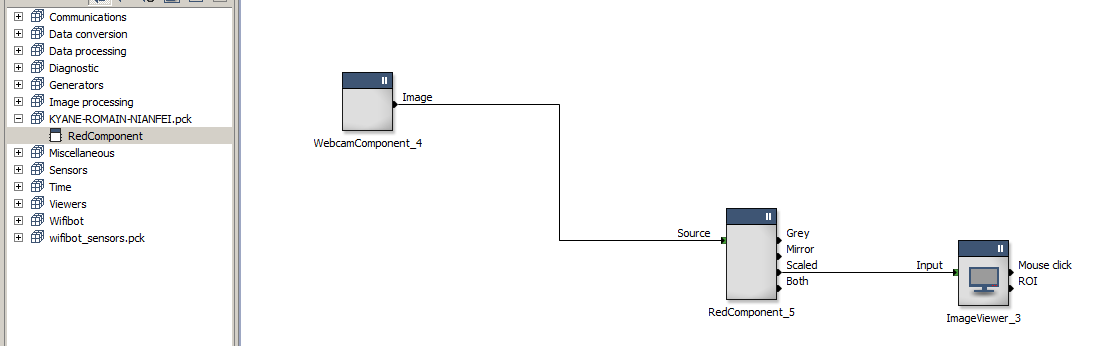
\includegraphics[width=1.0\textwidth]{pictures/screen.png}
   \caption{Module RTMaps}
\end{figure}

\section{Résultat visuel}

Voici nos 4 affichages en noir et blanc, de gauche à droite et de haut en bas :
\begin{itemize}
  \item Noir et blanc
  \item Miroir
  \item Noir et blanc selon 5 niveaux de gris
  \item Noir et blanc selon 5 niveaux de gris et miroir
\end{itemize}

\begin{figure}[!h]
   \centering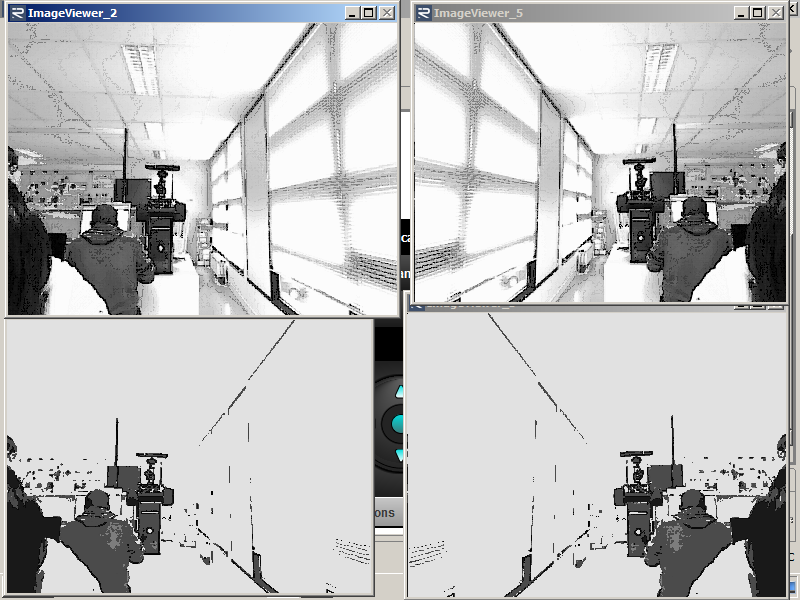
\includegraphics[width=1.0\textwidth]{pictures/noir_et_blanc.png}
   \caption{Les 4 affichages en noir et blanc}
\end{figure}

\section{Fichier .hpp}

Voici donc le code final de notre module RTMaps.
\begin{lstlisting}
#ifndef DEF_RED_COMPONENT_HPP
#define DEF_RED_COMPONENT_HPP

// Includes, rtmaps
#include "maps.hpp"

namespace sy31
{
  class RedComponent
    : public MAPSComponent
  {
    MAPS_COMPONENT_STANDARD_HEADER_CODE(RedComponent)
    protected:
      /// Allocate the output images.
      void allocateOutputs(IplImage const& src);

      /// Notre travail
     void fonction(IplImage const& src,IplImage & dst, bool scaled, bool mirror);

    private:
      bool mIsAllocated;
  };
}

#endif
\end{lstlisting}

\section{Fichier .cpp}
\begin{lstlisting}
// Includes, project
#include "red-component.hpp"

// Includes, standar
#include <cmath>

using namespace sy31;

////////////////////////////////////////////////////////////////
// RTMaps - Input
////////////////////////////////////////////////////////////////
MAPS_BEGIN_INPUTS_DEFINITION(RedComponent)
  MAPS_INPUT("Source", MAPS::FilterIplImage, MAPS::FifoReader)
MAPS_END_INPUTS_DEFINITION

////////////////////////////////////////////////////////////////
// RTMaps - Output
////////////////////////////////////////////////////////////////
MAPS_BEGIN_OUTPUTS_DEFINITION(RedComponent)
  MAPS_OUTPUT("Grey", MAPS::IplImage, NULL, NULL, 1)
  MAPS_OUTPUT("Mirror", MAPS::IplImage, NULL, NULL, 1)
  MAPS_OUTPUT("Scaled", MAPS::IplImage, NULL, NULL, 1)
  MAPS_OUTPUT("Both", MAPS::IplImage, NULL, NULL, 1)
MAPS_END_OUTPUTS_DEFINITION

////////////////////////////////////////////////////////////////
// RTMaps - Properties
////////////////////////////////////////////////////////////////
MAPS_BEGIN_PROPERTIES_DEFINITION(RedComponent)
MAPS_END_PROPERTIES_DEFINITION

////////////////////////////////////////////////////////////////
// RTMaps - Actions
////////////////////////////////////////////////////////////////
MAPS_BEGIN_ACTIONS_DEFINITION(RedComponent)
MAPS_END_ACTIONS_DEFINITION

////////////////////////////////////////////////////////////////
// RTMaps - Definition
////////////////////////////////////////////////////////////////
MAPS_COMPONENT_DEFINITION(
	RedComponent, "RedComponent", "1.0", 128,
	MAPS::Threaded|MAPS::Sequential,MAPS::Threaded,
  1, // Nb of inputs
	4, // Nb of outputs
	0, // Nb of properties
	0) // Nb of actions

void
RedComponent::Birth()
{
  mIsAllocated = false;
}

void
RedComponent::Core() 
{
  MAPSIOElt* input = StartReading(Input("Source"));
  IplImage& source = input->IplImage();
  if (!mIsAllocated)
    allocateOutputs(source);

  MAPSIOElt* outGrey    = StartWriting(Output("Grey"));
  MAPSIOElt* outScaled  = StartWriting(Output("Scaled"));
  MAPSIOElt* outMirror  = StartWriting(Output("Mirror"));
  MAPSIOElt* outBoth  = StartWriting(Output("Both"));

  IplImage& grey   = outGrey->IplImage();
  IplImage& scaled = outScaled->IplImage();
  IplImage& mirror = outMirror->IplImage();
  IplImage& both = outBoth->IplImage();

  /* Convertir l'image en niveaux de gris */
 fonction(source,grey,false,false);
 fonction(source,scaled,true,false);
 fonction(source,mirror,false,true);
 fonction(source,both,true,true);

  /* Set the timestamps */
  outGrey->Timestamp()  = MAPS::CurrentTime();
  outScaled->Timestamp()  = MAPS::CurrentTime();
  outMirror->Timestamp()  = MAPS::CurrentTime();
  outBoth->Timestamp()  = MAPS::CurrentTime();

  StopReading(Input("Source"));
  StopWriting(outGrey);
  StopWriting(outScaled);
  StopWriting(outMirror);
  StopWriting(outBoth);
}

void
RedComponent::Death()
{
  // Couic! :(
}

void
RedComponent::allocateOutputs(IplImage const& src)
{
  IplImage model = MAPS::IplImageModel(src.width, src.height, MAPS_CHANNELSEQ_GRAY);

  Output("Grey").AllocOutputBufferIplImage(model);
  Output("Scaled").AllocOutputBufferIplImage(model);
  Output("Mirror").AllocOutputBufferIplImage(model);
  Output("Both").AllocOutputBufferIplImage(model);

  mIsAllocated = true;
}

void
RedComponent::fonction(IplImage const& src,IplImage & dst, bool scaled, bool mirror)
{
	for(int i=0; i<src.width*src.height;i++) {

		int val = (src.imageData[3*i]*0.299) + (src.imageData[(3*i)+1]*0.587) + (src.imageData[(3*i)+2]*0.114);
		
		if (scaled) {
			if (val >=0 && val < 50)
				val = 25;
			else if (val >= 50 && val < 100)
				val = 75;
			else if (val >= 100 && val < 150)
				val = 125;
			else if (val >= 150 && val < 200)
				val = 175;
			else
				val = 225;
		}

		if (mirror)
			dst.imageData[((i/src.width)+1)*src.width-(i%src.width)] = val;
		else
			dst.imageData[i] = val;
	}
}
\end{lstlisting}

\chapter{Développement lors de la troisième séance}
\section{Affichage en couleurs}

Pour afficher une image en couleurs, il suffisait simplement de modifier la structure \lstinline{IplImage} comme ceci dans la fonction \lstinline{allocateOutputs(IplImage const& src)} :

\begin{lstlisting}
void
RedComponent::allocateOutputs(IplImage const& src)
{
  IplImage model = MAPS::IplImageModel(src.width, src.height, MAPS_CHANNELSEQ_BGR);
  Output("Color").AllocOutputBufferIplImage(model);
  mIsAllocated = true;
}
\end{lstlisting}
Il suffisait ensuite de modifier la fonction \lstinline{fonction(...)} utilisée précédemment comme ceci :
\begin{lstlisting}
void RedComponent::fonction(IplImage const& src,IplImage & dst)
{
  for(int i=0; i<src.width*src.height;i++) {

    int blue  = src.imageData[3*i];
    int green = src.imageData[3*i+1];
    int red   = src.imageData[3*i+2];
    
    dst.imageData[3*i] = blue;
    dst.imageData[3*i+1] = green;
    dst.imageData[3*i+2] = red;
  }
}
\end{lstlisting}

\section{Affichage en couleurs de la composante prédominante}
\begin{lstlisting}
void RedComponent::fonction(IplImage const& src,IplImage & dst)
{
  for(int i=0; i<src.width*src.height;i++) {

    int blue  = src.imageData[3*i];
    int green = src.imageData[3*i+1];
    int red   = src.imageData[3*i+2];
 
    dst.imageData[3*i] = (blue>=red)&&(blue>=green)?255:0;
    dst.imageData[3*i+1] = (green>=blue)&&(green>=red)?255:0;
    dst.imageData[3*i+2] = (red>=blue)&&(red>=green)?255:0;
  }
}
\end{lstlisting}

\section{Résultat visuel}

\begin{figure}[!h]
   \centering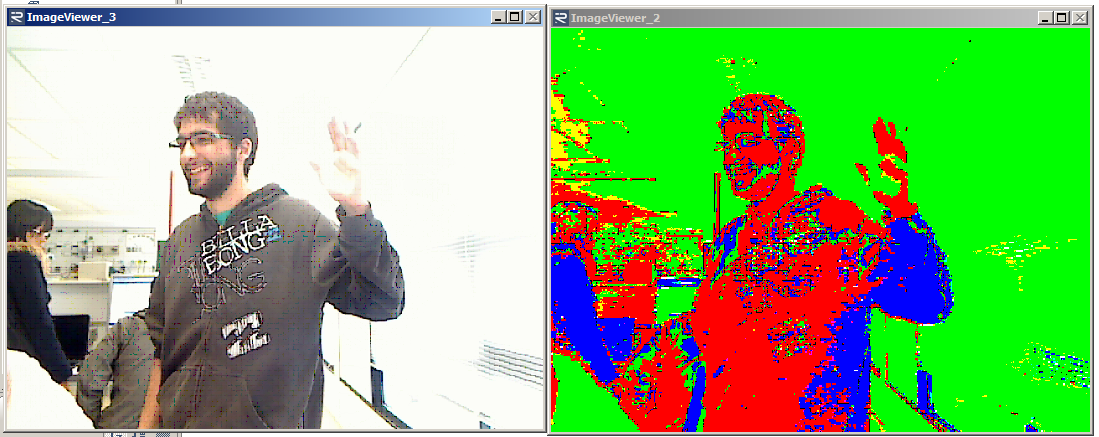
\includegraphics[width=1.0\textwidth]{pictures/couleurs.png}
   \caption{Affichages en couleur et de la prédominante}
\end{figure}

\end{document}
